% Exact source-layer transcription of Xi Yin, Physics 253a,
% original note pp. 10--29; combined source PDF physical pp. 21--40.
% Combined source PDF:
%   /Users/wlancer/Desktop/IAS/phy/qft/qft_253abc_book.pdf
% Source SHA-256:
%   9e5e4d241fffffa56c1c3df6dce4b83178f75787dd5d794a18c5d0c087769f21
%
% This is a literal note-layer capture. Source order, line fragments,
% punctuation, colors, arrows, braces, corrections, questions, and diagrams
% are retained. No source notation is silently normalized.
%
% Open source readings are tied to:
%   work/253a-ch02/ambiguities.md
%
% Compilation requirements for reconstructed diagrams:
%   xcolor, tikz, tikz libraries arrows.meta, positioning,
%   decorations.pathmorphing.

\providecommand{\YinPageBoundary}[2]{%
  \clearpage
  \noindent\textsf{[Original Physics 253a note p.~#1; combined PDF physical p.~#2]}%
  \par\medskip
}
\providecommand{\YinLine}[1]{\noindent #1\par}
\providecommand{\YinIndent}[1]{\noindent\hspace*{2em}#1\par}
\providecommand{\YinBullet}[1]{\noindent\hspace*{1em}$\bullet$\hspace{0.7em}#1\par}
\providecommand{\YinDash}[1]{\noindent\hspace*{1em}--\hspace{0.7em}#1\par}
\providecommand{\YinBlue}[1]{{\color[rgb]{0.00,0.34,0.92}#1}}
\providecommand{\YinLightBlue}[1]{{\color[rgb]{0.47,0.67,0.82}#1}}
\providecommand{\YinPurple}[1]{{\color[rgb]{0.61,0.16,0.88}#1}}
\providecommand{\YinGray}[1]{{\color[rgb]{0.58,0.58,0.58}#1}}
\providecommand{\YinGreen}[1]{{\color[rgb]{0.00,0.52,0.22}#1}}
\providecommand{\YinRed}[1]{{\color[rgb]{0.95,0.18,0.10}#1}}
\providecommand{\YinMagenta}[1]{{\color[rgb]{0.75,0.00,0.55}#1}}
\providecommand{\YinOrange}[1]{{\color[rgb]{0.95,0.43,0.00}#1}}
\providecommand{\ket}[1]{\lvert #1\rangle}
\providecommand{\bra}[1]{\langle #1\rvert}
\providecommand{\braket}[2]{\langle #1\mid #2\rangle}

% ---------------------------------------------------------------------------
\YinPageBoundary{10}{21}

\YinLine{\underline{Lagrangian formalism}}
\YinLine{Recall in classical mechanics:}

% The source is a two-column comparison. The blue U-shaped connector has
% arrowheads at both rising ends and the words related by below it.
\begin{center}
\begin{tikzpicture}[
  x=1cm,y=1cm,
  every node/.style={font=\small},
  >=Stealth
]
  \node (lag) at (-4.1,0) {Lagrangian};
  \node (vs) at (0,0) {vs};
  \node (ham) at (4.1,0) {Hamiltonian};

  \node[anchor=north west,align=left] at (-6.1,-0.55) {%
    \text{\textquotedblleft state\textquotedblright}\hspace{1.6em} $q,\dot q$};
  \node[anchor=north west,align=left] at (1.9,-0.55) {%
    $q,p.$};

  \node[anchor=north west,align=left] at (-6.1,-1.45) {%
    EOM\hspace{2.2em} extremize};
  \node[anchor=north west,align=left] at (1.9,-1.45) {%
    $\dot f=\{H,f\}_{\mathrm{Poisson}}$};

  \node[anchor=north west,align=left] at (-2.1,-2.35) {%
    $S=\displaystyle\int dt\,L(q,\dot q)$};
  \node[anchor=north west,align=left,text=gray] at (1.85,-2.35) {%
    \begin{gathered}
      \text{\YinGray{e.g.}}\quad
      \dot q=\dfrac{\partial H}{\partial p},\\[3pt]
      \dot p=-\dfrac{\partial H}{\partial q}.
    \end{gathered}};

  \draw[blue,->,line width=0.85pt]
    (-3.2,-3.1) .. controls (-3.2,-4.15) and (3.2,-4.15) .. (3.2,-3.1);
  \draw[blue,->,line width=0.85pt]
    (3.2,-3.1) .. controls (3.2,-4.15) and (-3.2,-4.15) .. (-3.2,-3.1);
  \node[blue] at (0,-4.28) {related by};
  \node[blue,align=center] at (0,-5.05) {%
    $\displaystyle H(p,q)=
      \left.p\dot q-L(q,\dot q)\right|_{\frac{\partial L}{\partial\dot q}=p}$};

  \draw[blue,dashed,line width=0.7pt] (0,-5.45) -- (0,-10.8);
  \node[anchor=west] at (-6.1,-6.05) {QM:};
  \node at (-3.9,-6.05) {Hamiltonian};
  \node at (0,-6.05) {vs};
  \node at (3.8,-6.05) {Lagrangian};

  \node[anchor=north west,align=left] at (-6.1,-6.55) {%
    State\hspace{1.25em} $|\psi\rangle\in\mathcal H$\\[5pt]
    \hspace*{1.5em}$H(p,q)\leadsto\hat H$};
  \node[anchor=north west] at (1.9,-6.55) {%
    $\displaystyle S=\int dt\,L(q,\dot q)$};
\end{tikzpicture}
\end{center}

% PAGE-TRANSITION: physical p. 21 closes the classical comparison and begins
% the quantum-mechanics comparison at the lower margin.

% ---------------------------------------------------------------------------
\YinPageBoundary{11}{22}

% The upper half is a two-column comparison separated by a blue dashed line.
\begin{center}
\begin{tikzpicture}[
  every node/.style={font=\small},
  >=Stealth
]
  \node[anchor=north west,align=left] at (-7.2,0) {%
    time\\[-1pt] evolution};
  \draw[blue,dashed,line width=0.75pt] (0.0,0.2) -- (0.0,-5.6);

  \node[anchor=north west,align=left] at (-5.95,0) {%
    Schr\"odinger:\\[5pt]
    $\displaystyle|\psi\rangle\mapsto U(t)|\psi\rangle,$\\[7pt]
    $\displaystyle U(t)=e^{-\frac{i}{\hbar}\hat Ht}$\\[10pt]
    Heisenberg:\\[5pt]
    $\displaystyle O\mapsto
      \underbrace{(U(t))^{-1}OU(t)}_{
        \YinBlue{\substack{\text{|||}\\[-3pt]O(t)}}}.$\\[8pt]
    $\displaystyle\dot O(t)=\frac{i}{\hbar}[\hat H,O(t)]$};

  \node[anchor=north west,align=left] at (0.55,0) {%
    $\displaystyle\langle q_f|U(T)|q_i\rangle$\\[7pt]
    $\displaystyle=
      \int_{q(0)=q_i}^{q(T)=q_f}[Dq]\,
      e^{\frac{i}{\hbar}S}$};
\end{tikzpicture}
\end{center}

% AMBIGUITY P22-A1: three short blue marks above O(t) under the Heisenberg
% underbrace have no settled symbolic reading. See
% work/253a-ch02/ambiguities.md.

\begin{center}
\begin{tikzpicture}[baseline,>=Stealth]
  \node (measure) {$[Dq]$};
  \draw[magenta,line width=0.8pt,decorate,
    decoration={snake,amplitude=0.30mm,segment length=1.8mm}]
    (measure.south west) -- (measure.south east);
  \draw[magenta,->,line width=0.8pt]
    (measure.north) to[out=100,in=-90] (0.3,1.0);
  \node[magenta,anchor=west] at (0.38,1.0) {what is this ?};
\end{tikzpicture}
\end{center}

\YinBullet{Much of the subtleties with the Lagrangian
  formulation of QM have to do with the
  path integral measure [Dq].}
\YinLine{Let us revisit its derivation:}
\YinLine{Consider the time evolution by T}
\YinIndent{in N steps,}

\begin{center}
\begin{tikzpicture}[x=1cm,y=1cm,>=Stealth,every node/.style={font=\small}]
  \draw[line width=0.7pt] (-5,0) -- (5,0);
  \foreach \x/\lab in {-5/$q_i$,-3.35/$q_1$,-1.70/$q_2$,
                         0/$q_3$,1.65/$\cdots$,3.25/$q_{N-1}$,5/$q_f$} {
    \draw[line width=0.7pt] (\x,-0.10) -- (\x,0.10);
    \node[above=2pt] at (\x,0.10) {\lab};
  }
  \node[below=5pt] at (-5,0) {0};
  \node[below=5pt] at (5,0) {T};
  \draw[blue,line width=0.75pt,decorate,
    decoration={brace,amplitude=4pt,mirror}]
    (-5,-0.28) -- (-3.35,-0.28);
  \node[blue,below=9pt] at (-4.18,-0.28) {T/N};
\end{tikzpicture}
\end{center}

% PAGE-TRANSITION: the time-slicing diagram reaches the lower margin as an
% open derivation boundary. The next page inserts position and momentum
% resolutions and expands the short-time Hamiltonian factors.

% ---------------------------------------------------------------------------
\YinPageBoundary{12}{23}

\[
 \langle q_f\mid U(T)\mid q_i\rangle
\]
\[
\begin{aligned}
={}&\int d^Dq_1\,\cdots\,d^Dq_{N-1}\,
 \langle q_f\mid e^{-\frac{i}{\hbar}\hat H\,\cdot\,\frac{T}{N}}
       \mid q_{N-1}\rangle
 \,\cdots\,
 \langle q_1\mid e^{-\frac{i}{\hbar}\hat H\,\cdot\,\frac{T}{N}}
       \mid q_i\rangle
\end{aligned}
\]
\YinLine{\YinBlue{[ denote $q_f\equiv q_N,\qquad q_i\equiv q_0$ ]}}
\[
\begin{aligned}
={}&\int\prod_{n=1}^{N-1}d^Dq_n\;\cdot\;
 \prod_{n=0}^{N-1}
 \langle q_{n+1}\mid
 e^{-\frac{i}{\hbar}\hat H\,\cdot\,\frac{T}{N}}
 \mid q_n\rangle .
\end{aligned}
\]

% The long blue curved arrow selects one short-time factor and inserts the
% momentum resolution shown below.
\begin{center}
\begin{tikzpicture}[baseline,>=Stealth]
  \node (from) at (-2.2,0)
    {$\prod\langle q_{n+1}\mid e^{-\frac{i}{\hbar}\hat H\frac{T}{N}}
       \mid q_n\rangle$};
  \node[blue,anchor=west] (to) at (1.2,-0.55)
    {$\displaystyle\int\frac{d^Dp_n}{(2\pi\hbar)^D}
      \langle q_{n+1}\mid p_n\rangle
      \langle p_n\mid e^{-\frac{i}{\hbar}\hat H\frac{T}{N}}
      \mid q_n\rangle$};
  \draw[blue,->,line width=0.8pt]
    (from.south east) to[out=-25,in=145] (to.north west);
\end{tikzpicture}
\end{center}

\[
\YinBlue{%
\begin{aligned}
 &\underbrace{\langle q_{n+1}\mid p_n\rangle}_{\text{\scriptsize two short strokes}}\\[-2pt]
 &\hspace{4em}
 =e^{\frac{i}{\hbar}p_n\cdot q_{n+1}}
\end{aligned}}
\qquad
\YinBlue{%
\underbrace{\left\langle p_n\middle|
 e^{-\frac{i}{\hbar}\hat H\,\frac{T}{N}}\middle|q_n\right\rangle}_{
 \YinBlue{\scriptstyle\text{\raisebox{1pt}{\(\approx\!\approx\)}}}}
 \approx
 e^{-\frac{i}{\hbar}H(q_n,p_n)\frac{T}{N}}
 e^{-\frac{i}{\hbar}p_n\cdot q_n}}
\]

\YinLine{\YinMagenta{classical Hamiltonian}
  \hspace{1em}\YinMagenta{$\uparrow$}\hspace{1em}
  $H(q_n,p_n)$}
\[
\begin{aligned}
={}&\int\prod_{n=1}^{N-1}d^Dq_n
 \prod_{n=0}^{N-1}\frac{d^Dp_n}{(2\pi\hbar)^D}\\[-2pt]
&\quad\cdot\exp\left\{
 \frac{i}{\hbar}\sum_{n=0}^{N-1}
 \left[
 p_n\cdot(q_{n+1}-q_n)
 -H(q_n,p_n)\frac{T}{N}
 +O\left(\hbar,\left(\frac{T}{N}\right)^2\right)
 \right]\right\}.
\end{aligned}
\]

% AMBIGUITY P23-A1: the first blue underbrace has a small mark resembling
% 11 and the second has a double-wavy mark resembling an approximation sign
% or an unreadable label. See work/253a-ch02/ambiguities.md.
% AMBIGUITY P23-A2: the source uses the visible O-term glyph captured as
% O(hbar,(T/N)^2). No higher-layer normalization is made here.

% PAGE-TRANSITION: physical p. 23 closes with the finite-N phase-space
% expression and its O(hbar,(T/N)^2)-type remainder. Physical p. 24 takes
% the formal N to infinity limit.

% ---------------------------------------------------------------------------
\YinPageBoundary{13}{24}

\YinLine{\text{formally, in }N\to\infty\
  \text{\textquotedblleft limit\textquotedblright}}
\[
\begin{aligned}
={}&\int\mathcal Dq\,\mathcal Dp\;
 e^{\frac{i}{\hbar}\int_0^Tdt\,(p\cdot\dot q-H(q,p))}.
\end{aligned}
\]
\begin{center}
\begin{tikzpicture}[baseline,>=Stealth,every node/.style={font=\small}]
  \node (measure) {$\mathcal Dq\,\mathcal Dp$};
  \node[blue,align=left,anchor=west] (reg) at (1.4,0.05) {%
    defined via\\[-1pt] regularization\\[-1pt] e.g. discretizing time};
  \draw[blue,->,line width=0.75pt]
    (measure.south) to[out=-80,in=170] (reg.west);
  \node (h) at (0,-1.0) {$H(q,p)$};
  \node[blue,align=left,anchor=west] (amb) at (1.4,-1.0) {%
    Contains $O(\hbar)$ ambiguities\\[-1pt]
    -- \textquotedblleft counter terms\textquotedblright\\[-1pt]
    -- these ambiguities\\[-1pt]
    \hspace*{1em}are tied to the scheme\\[-1pt]
    \hspace*{1em}of regularization.};
  \draw[blue,->,line width=0.75pt]
    (h.east) to[out=0,in=180] (amb.west);
\end{tikzpicture}
\end{center}

% AMBIGUITY P24-A1: the handwritten O glyph resembles a small t with an
% h-like component. The exact-layer capture uses O(hbar). See
% work/253a-ch02/ambiguities.md.
\YinLine{\YinGray{An example of alternative time-lattice regularization:}}
\[
\YinGray{%
\int_0^Tdt\;p\cdot\dot q
\longrightarrow
\sum_{n=0}^{N-1}p_n\cdot(q_{n+1}-q_n)}
\]
\[
\YinGray{\text{versus}\qquad
\sum_{n=0}^{N-1}p_{n+1}\cdot(q_{n+1}-q_n)}
\]
\YinLine{\YinGray{The exact representation of the time evolution is}}
\[
\YinGray{%
\cdots\,\langle q_{n+1}\mid p_n\rangle
\langle p_n\mid e^{-\frac{i}{\hbar}\hat H\,\frac{T}{N}}
\mid q_n\rangle\,\cdots}
\]
\YinLine{\YinGray{in the former case, and}}
\[
\YinGray{%
\langle p_n\mid\hat H\mid q_n\rangle
=H(p_n,q_n)\langle p_n\mid q_n\rangle}
\]
\[
\YinBlue{%
\cdots\,\langle p_{n+1}\mid q_n\rangle
\langle q_n\mid e^{-\frac{i}{\hbar}\hat H\,\frac{T}{N}}
\mid p_n\rangle\,\cdots}
\]
\YinLine{\YinBlue{in the latter case}}
\[
\YinBlue{%
\langle q_n\mid\hat H\mid p_n\rangle
=H'(p_n,q_n)\langle q_n\mid p_n\rangle}
\]
\YinLine{%
  \YinPurple{$H(p_n,q_n)$}\ \text{and}\
  \YinBlue{$H'(p_n,q_n)$}\ \text{can differ at order }O(\hbar).}

% AMBIGUITY P24-A2: preserve H(q_n,p_n) in the finite-N exponent on p. 23,
% H(p_n,q_n) in the purple relation here, and H'(p_n,q_n) in the blue
% relation. See work/253a-ch02/ambiguities.md.
% PAGE-TRANSITION: physical p. 24 hands off the regularization discussion
% to the Gaussian momentum-integration case beginning on physical p. 25.

% ---------------------------------------------------------------------------
\YinPageBoundary{14}{25}

\YinLine{If $H(q,p)$ is quadratic in $p$.}
\YinLine{\YinGray{e.g.}\quad
  $H(q,p)=\dfrac{p^2}{2m}+V(q)$,}
\YinLine{we can integrate out $P(t)$ as Gaussian,}
\YinLine{leaving}
\[
\int[D\xi]\,
 e^{\frac{i}{\hbar}\int_0^Tdt\,(p\dot\xi-H)}
\bigg|_{\dot\xi=\frac{\partial H}{\partial p}}
\]
\begin{center}
\begin{tikzpicture}[baseline,>=Stealth,every node/.style={font=\small}]
  \node (measure) {$[D\xi]$};
  \node[blue,align=left,anchor=west] (det) at (1.4,0) {%
    absorbs Gaussian\\[-1pt] determinant of $P(t)$};
  \draw[blue,->,line width=0.75pt]
    (det.west) to[out=180,in=0] (measure.east);
\end{tikzpicture}
\end{center}
\begin{center}
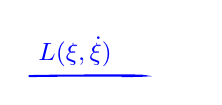
\begin{tikzpicture}[baseline,every node/.style={font=\small}]
  \node[blue] (laglabel) {$L(\xi,\dot\xi)$};
  \draw[blue,line width=0.75pt]
    (laglabel.south west) .. controls (-0.2,-0.3) and (1.5,-0.3) ..
    (laglabel.south east);
\end{tikzpicture}
\end{center}
\YinLine{\YinGray{More generally, Lagrangian in generalized coordinates}}
\YinLine{\YinGray{typically takes the form}}
\[
\YinGray{%
L=\frac{1}{2}G_{\alpha\beta}(\xi)\dot\xi^\alpha\dot\xi^\beta-V(\xi)}
\qquad
\YinGray{\left[\begin{array}{l}
\text{e.g. rotating}\\[-1pt]
\text{3D rigid body}
\end{array}\right]}
\]
\[
\YinGray{%
\Longleftrightarrow\quad
H=\frac{1}{2}\bigl(G^{-1}(\xi)\bigr)^{\alpha\beta}p_\alpha p_\beta
  +V(\xi)+\YinLightBlue{O(\hbar)}}
\]
\YinLine{\YinGray{Path integral}}
\[
\YinGray{%
\int\mathcal Dp\,\mathcal D\xi\,
e^{\frac{i}{\hbar}\int dt\,
(p_\alpha\dot\xi^\alpha-H(p,\xi))}
=
\int[D\xi]\,
e^{\frac{i}{\hbar}\int dt\,L(\xi,\dot\xi)}}
\]
\[
\YinGray{%
[D\xi]\;\leadsto\;
\prod_{n=1}^{\widetilde N}
\frac{d\xi_n^\alpha}
{\sqrt{2\pi i\hbar\,\frac{T}{N}}}
\sqrt{\det G_{\alpha\beta}(\xi_n)}\, .}
\]

% AMBIGUITY P25-A1: the source prose and determinant note visibly use P(t),
% while the phase-space equations use p. Preserve the visible P(t). See
% work/253a-ch02/ambiguities.md.
% AMBIGUITY P25-A2: the handwritten Dp Dxi measures do not settle
% calligraphic status or differential subscripts. The source-layer surrogate
% above preserves the visible measure variables.
% AMBIGUITY P25-A3: xi is retained as the generalized-coordinate glyph.
% AMBIGUITY P25-A4: the pale-blue correction is captured as +O(hbar).
% AMBIGUITY P25-A5: the product upper limit has a tilde, while the square
% root visibly contains T/N. Both forms are kept.
% AMBIGUITY P25-A6: the evaluation bar is placed after the full displayed
% phase-space factor as visually reported. See work/253a-ch02/ambiguities.md.
% PAGE-TRANSITION: physical p. 25 ends after the discretized measure.
% Physical p. 26 begins a new correlation-function bullet.

% ---------------------------------------------------------------------------
\YinPageBoundary{15}{26}

% The leading dot is a source mark at the left margin.
\YinLine{. Consider correlation function in}
\YinIndent{ground state $|0\rangle$, \quad e.g.}
\[
G(t)\equiv\langle 0|\hat q_{\beta}(t)\,\hat q_{\beta}(0)|0\rangle
\]
\[
=\sum_n\langle 0|\hat q_{\beta}(t)|n\rangle
  \langle n|\hat q_{\beta}(0)|0\rangle
\]
\begin{center}
\begin{tikzpicture}[baseline,>=Stealth,every node/.style={font=\small}]
  \node (state) {$|n\rangle$};
  \draw[blue,line width=0.75pt,decorate,
    decoration={snake,amplitude=0.28mm,segment length=1.8mm}]
    (state.south west) -- (state.south east);
  \node[blue,anchor=west] (basis) at (0.85,0.15)
    {a basis of $\hat H$ - eigenstates};
  \draw[blue,->,line width=0.75pt]
    (state.north east) to[out=45,in=180] (basis.west);
\end{tikzpicture}
\end{center}
\[
\YinBlue{\hat H|n\rangle=E_n|n\rangle.}
\]
\[
\begin{aligned}
=\sum_n\,
\langle 0|e^{\YinBlue{\frac{i}{\hbar}}\hat Ht}
\hat q_{\beta}(0)e^{-\YinBlue{\frac{i}{\hbar}}\hat Ht}|n\rangle
\langle n|\hat q_{\beta}(0)|0\rangle
\end{aligned}
\]
\[
\begin{aligned}
=\sum_n\,
\langle 0|\hat q_{\beta}(0)|n\rangle
\langle n|\hat q_{\beta}(0)|0\rangle\,\cdot\,
e^{-\frac{i}{\hbar}(E_n-E_0)t}.
\end{aligned}
\]
\[
\underbrace{%
\langle 0|\hat q_{\beta}(0)|n\rangle
\langle n|\hat q_{\beta}(0)|0\rangle%
}_{\YinBlue{\substack{\text{\scriptsize |||}\\[-2pt]\beta_n,\ \text{some number}}}}
\]
\YinLine{As $E_n-E_0>0$, can analytically continue}
\YinLine{$G(t)$ as a function of complex $t$,}
\YinLine{provided $\operatorname{Im}t<0$. So that $\sum_n$ converges.}
\YinLine{\YinGray{[Paley-Wiener theorem]}}

% AMBIGUITY P26-A1: the blue coefficient label is captured as beta_n, with
% a possible cursive g_n reading for its first glyph. See
% work/253a-ch02/ambiguities.md.
% AMBIGUITY P26-A2: blue accents on the i/hbar factors are retained as
% source annotations; their editing chronology is unresolved.
% AMBIGUITY P26-A3: the leading margin dot before Consider is preserved as
% a source mark.
% PAGE-TRANSITION: physical p. 26 ends with the strict lower-half-plane
% convergence statement and the gray Paley-Wiener cue. Physical p. 27
% begins with t=-i tau and the quoted Wick rotation label.

% ---------------------------------------------------------------------------
\YinPageBoundary{16}{27}

\YinLine{e.g. \quad $t=-i\tau,\quad\tau\in\mathbb R_+$}
\YinLine{\text{\textquotedblleft Wick rotation\textquotedblright}}
\[
\langle 0|\hat q(t)\hat q(0)|0\rangle
=\sum_n
\langle 0|\hat q(0)|n\rangle
\langle n|\hat q(0)|0\rangle
\cdot e^{-\YinBlue{\frac{1}{\hbar}}(E_n-E_0)\tau}.
\]
\YinLine{Assuming a gap $\bar E_1-\bar E_0>0$, \quad can replace}
\YinLine{$|0\rangle$ \quad by\quad
  $\displaystyle\lim_{T\to\infty}
  e^{-\YinBlue{\frac{1}{\hbar}}(\hat H-E_0)T}|\psi\rangle,$}
\YinLine{up to overall normalization,}
\YinLine{for any generic state $|\psi\rangle$.}
\YinLine{\YinGray{(that has nonzero overlap with $|0\rangle$)}}
\[
\langle 0|\hat q(t)\hat q(0)|0\rangle
=\lim_{T\to\infty}
\frac{%
\langle\psi|
\underbrace{e^{-\YinBlue{\frac{1}{\hbar}}\hat H T}}_{\YinPurple{\text{\scriptsize left brace}}}
\hat q(t)\hat q(0)
\underbrace{e^{-\YinBlue{\frac{1}{\hbar}}\hat H T}}_{\YinBlue{\text{\scriptsize right brace}}}
|\psi\rangle}{%
\langle\psi|e^{-\YinBlue{\frac{2}{\hbar}}\hat H T}|\psi\rangle}.
\]
\YinLine{\YinRed{$\downarrow$ to $\hat q(t)$}\hspace{3em}
  \YinOrange{$\downarrow$ to $\hat q(0)$}}

\begin{center}
\begin{tikzpicture}[x=1cm,y=1cm,>=Stealth,every node/.style={font=\small}]
  \draw[->,line width=0.75pt] (-2.8,0) -- (3.8,0)
    node[right] {Re $t$};
  \draw[->,line width=0.75pt] (-2.0,-1.2) -- (-2.0,4.1)
    node[above] {-Im $t$};
  \draw[magenta,line width=1.1pt] (-2.0,0) -- (-2.0,3.15);
  \draw[magenta,->,line width=0.95pt] (-2.0,2.2) -- (-2.0,2.8);
  \draw[blue,line width=1.0pt] (-2.0,-1.0) -- (-2.0,0.25);
  \draw[blue,->,line width=0.9pt] (-2.0,-0.55) -- (-2.0,-0.05);
  \draw[green!55!black,line width=1.0pt]
    (-2.0,3.15) .. controls (-0.6,3.1) and (1.5,2.6) .. (2.7,1.0);
  \draw[green!55!black,line width=1.0pt]
    (-2.0,0.25) .. controls (-0.8,0.45) and (1.4,1.5) .. (2.7,1.0);
  \draw[green!55!black,->,line width=0.85pt]
    (1.5,0.95) -- (2.0,1.0);
  \fill[orange] (-2.0,0.25) circle (2.6pt);
  \fill[red] (2.7,1.0) circle (2.8pt);
\end{tikzpicture}
\end{center}

% AMBIGUITY P27-A1: the gap accents are horizontal bars, captured as
% bar E_1 minus bar E_0. The p. 27 contour has two green traces; only the
% lower one has a separately visible rightward arrow.
% PAGE-TRANSITION: physical p. 27 closes with the complex-t contour sketch.
% Physical p. 28 begins with Alternatively, and a straight Euclidean-time
% representation.

% ---------------------------------------------------------------------------
\YinPageBoundary{17}{28}

\YinLine{Alternatively,}
\[
G(t=-i\tau)
=\langle 0|e^{\YinBlue{\frac{1}{\hbar}}H\tau}
\hat q(0)e^{-\YinBlue{\frac{1}{\hbar}}H\tau}
\hat q(0)|0\rangle.
\]
\[
\begin{aligned}
G(t=-i\tau)
={}&\lim_{T\to\infty}
\frac{%
\langle\psi|
e^{-\YinBlue{\frac{1}{\hbar}}H(T-\tau)}
\hat q(0)
e^{-\YinBlue{\frac{1}{\hbar}}H\tau}
q(0)
e^{-\YinBlue{\frac{1}{\hbar}}HT}
|\psi\rangle}{%
\langle\psi|e^{-\YinBlue{\frac{2}{\hbar}}HT}|\psi\rangle}.
\end{aligned}
\]
\YinLine{\YinRed{$\downarrow$ to the first insertion}
  \hspace{3em}\YinOrange{$\downarrow$ to the second insertion}}

\begin{center}
\begin{tikzpicture}[x=1cm,y=1cm,>=Stealth,every node/.style={font=\small}]
  \draw[blue,line width=1.0pt] (-4.4,0) -- (1.7,0);
  \draw[black,->,line width=0.75pt] (1.7,0) -- (4.0,0)
    node[right] {-Im $t$};
  \draw[blue,line width=0.9pt] (-4.4,-0.16) -- (-4.4,0.16);
  \draw[blue,line width=0.9pt] (1.7,-0.16) -- (1.7,0.16);
  \fill[orange] (-1.9,0) circle (2.6pt);
  \fill[red] (-0.05,0) circle (2.6pt);
  \node[blue,below=3pt] at (-4.4,0) {-T};
  \node[orange,below=3pt] at (-1.9,0) {0};
  \node[red,below=3pt] at (-0.05,0) {$\tau$};
  \node[blue,below=3pt] at (1.7,0) {T};
\end{tikzpicture}
\end{center}

\YinLine{From path integral:}
\[
\langle 0|\hat q(t)\hat q(0)|0\rangle
=\lim_{\substack{\operatorname{Im}t_f\to-\infty\\
                  \operatorname{Im}t_i\to+\infty}}
\frac{%
\displaystyle\int[Dq]\,
e^{\frac{i}{\hbar}\int_{t_i}^{t_f}L[q,\dot q]\,dt}\,
q(t)\,q(0)\,\text{.}}{%
\displaystyle\int[Dq]\,
e^{\frac{i}{\hbar}\int_{t_i}^{t_f}L[q,\dot q]}}
\]
\YinLine{Wick rotation:}
\[
q(t)\mathrel{\overset{t=-i\tau}{\rightsquigarrow}}q(\tau).
\]

% AMBIGUITY P28-A1: the first top-line Euclidean exponential has no written
% leading minus sign. The source capture keeps its positive exponent.
% AMBIGUITY P28-A2: the second insertion in the large-T numerator is visibly
% q(0), while the top line has q-hats at both positions. See
% work/253a-ch02/ambiguities.md.
% AMBIGUITY P28-A3: the path-integral denominator omits the dt visible in
% the numerator. The omission is retained.
% PAGE-TRANSITION: physical p. 28 closes with the labeled map q(t) to q(tau).
% Physical p. 29 begins with the blue note still use the same notation and
% the derivative relation for the Wick-rotated variable.

% ---------------------------------------------------------------------------
\YinPageBoundary{18}{29}

\begin{center}
\begin{tikzpicture}[baseline,>=Stealth,every node/.style={font=\small}]
  \node[blue,anchor=west] (note) at (-1.4,0) {still use the same notation};
  \draw[blue,->,line width=0.75pt]
    (note.north west) to[out=120,in=-80] (-1.6,1.0);
\end{tikzpicture}
\end{center}
\[
\partial_t\dot q=+i\partial_\tau\dot q.
\]
\YinLine{Define}
\[
L[q,\dot q]\equiv-L^E[q,\partial_\tau q]
\]
\YinLine{so that}
\[
e^{\YinBlue{\frac{i}{\hbar}}\int L[q,\dot q]\,dt}
\rightsquigarrow
e^{\YinBlue{-\frac{1}{\hbar}}\int L^E[q,\partial_\tau q]\,d\tau}
\]
\[
\YinBlue{\underbrace{\hspace{5em}}_{S^E}}
\]
\YinLine{e.g.}
\[
L[q,\dot q]=\frac{1}{2}\dot q^2-V(q)
\]
\[
L^E[q,\partial_\tau q]=\frac{1}{2}(\partial_\tau q)^2+V(q)
\]
\YinBullet{How do we evaluate the path integral?}
\YinLine{the key is to find a convenient regularized}
\YinIndent{expression of the measure [Dq].}
\YinLine{e.g.}
\[
q(\tau)=\sum_n q_n f_n(\tau)
\]
\begin{center}
\begin{tikzpicture}[baseline,>=Stealth,every node/.style={font=\small}]
  \node (fn) {$f_n(\tau)$};
  \draw[blue,line width=0.75pt,decorate,
    decoration={snake,amplitude=0.28mm,segment length=1.8mm}]
    (fn.south west) -- (fn.south east);
  \draw[blue,->,line width=0.75pt]
    (fn.north) to[out=100,in=-90] (1.1,0.9);
  \node[blue,align=left,anchor=west] at (1.18,0.9)
    {a suitable basis of\\functions};
\end{tikzpicture}
\end{center}
\[
[Dq]\rightsquigarrow\prod_{n=1}^{\infty}dq_n\ ?
\]

% AMBIGUITY P29-A1: the blue phrase still use the same notation is a
% carry-forward annotation, not a new body-text sentence.
% AMBIGUITY P29-A2: the page-29 mode sum has a lower n and no recoverable
% upper limit. Physical p. 30 supplies the explicit n=1 to infinity form.
% AMBIGUITY P29-A3: the blue i/hbar and minus-one-over-hbar marks in the
% Wick-rotation exponents may be source corrections or emphasis.
% PAGE-TRANSITION: physical p. 29 ends with the open measure question.
% Physical p. 30 begins Example 1 and applies it to the harmonic oscillator.

% ---------------------------------------------------------------------------
\YinPageBoundary{19}{30}

\YinLine{\underline{Example 1:}}
\[
H=\frac{p^2+\omega^2q^2}{2}
\longleftrightarrow
L=\frac{1}{2}\dot q^2-\frac{1}{2}\omega^2q^2.
\]
\YinLine{Wick rotation $t=-i\tau$}
\YinLine{To evaluate}
\[
\int[Dq]e^{-\frac{1}{\hbar}S^E}\ \text{....}
\]
\YinLine{choose boundary condition in imaginary time}
\YinLine{e.g. $q(-T)=q(T)=0$ .}

\begin{center}
\begin{tikzpicture}[x=1cm,y=1cm,>=Stealth,every node/.style={font=\small}]
  \draw[->,line width=0.7pt] (-4.3,0) -- (4.5,0)
    node[right] {$\tau$};
  \draw[->,line width=0.7pt] (0,-2.2) -- (0,2.8)
    node[above] {$q(\tau)$};
  \draw[blue,line width=0.8pt] (-3.8,-0.12) -- (-3.8,0.12);
  \draw[blue,line width=0.8pt] (3.8,-0.12) -- (3.8,0.12);
  \node[blue,below=3pt] at (-3.8,0) {-T};
  \node[blue,below=3pt] at (3.8,0) {T};
  \draw[violet,line width=1.0pt]
    (-3.8,0)
    .. controls (-3.2,1.2) and (-2.6,1.0) .. (-2.3,0.25)
    .. controls (-2.0,-1.3) and (-1.5,-1.5) .. (-0.9,-0.45)
    .. controls (-0.3,0.75) and (0.35,1.4) .. (1.0,0.8)
    .. controls (1.55,0.1) and (1.8,1.0) .. (2.1,0.75)
    .. controls (2.7,0.35) and (2.95,0.1) .. (3.35,0.18)
    .. controls (3.55,0.15) and (3.7,0.05) .. (3.8,0);
\end{tikzpicture}
\end{center}
\YinLine{Expand $q(\tau)$ on a Fourier basis}
\[
q(\tau)=\sum_{n=1}^{\infty}q_n f_n(\tau)
\]
\begin{center}
\begin{tikzpicture}[baseline,>=Stealth,every node/.style={font=\small}]
  \node (fn) {$f_n(\tau)$};
  \draw[blue,->,line width=0.75pt]
    (fn.north) to[out=100,in=-80] (0.5,0.8);
\end{tikzpicture}
\end{center}
\[
\YinBlue{f_n(\tau)=\frac{1}{\sqrt{T}}
  \sin\frac{n\pi(\tau+T)}{2T}}
\]

% The purple curve is qualitative in the source and is not a prescribed
% function. The four visible dots after S^E are retained literally.
% AMBIGUITY P30-A1: the graph path is qualitative; only its zero endpoints
% and visible shape are source data.
% AMBIGUITY P30-A2: the path-integral continuation has four visible dots,
% captured as \text{....}. See work/253a-ch02/ambiguities.md.
% PAGE-TRANSITION: physical p. 30 ends with the blue Fourier basis formula.
% Physical p. 31 explains its boundary-adapted orthonormality and
% diagonalizes the oscillator action.

% ---------------------------------------------------------------------------
\YinPageBoundary{20}{31}

\YinBullet{$f_n(\tau)$ is a basis of functions that
  obeys the prescribed boundary condition,
  orthonormal with respect to a suitable
  inner product, e.g.}
\[
(f_n,f_m):=\int_{-T}^{T}f_n^*(\tau)f_m(\tau)\,d\tau=\delta_{nm}.
\]
\YinLine{and, for convenience, diagonalize the}
\YinIndent{kinetic term in the action:}
\[
\begin{aligned}
S^E
={}&\int_{-T}^{T}
\left[\frac{1}{2}(\partial_\tau q)^2+\frac{1}{2}\omega^2q^2\right]\,d\tau\\
={}&\sum_{n=1}^{\infty}
\left[\frac{1}{2}\left(\frac{n\pi}{2T}\right)^2
+\frac{1}{2}\omega^2\right]q_n^2.
\end{aligned}
\]
\[
\int[Dq]e^{-\frac{1}{\hbar}S^E}\cdots
\rightsquigarrow
\int\prod_{n=1}^{\infty}dq_n\,
\underbrace{e^{-\frac{1}{\hbar}\sum_{n=1}^{\infty}
\frac{1}{2}\left[\left(\frac{n\pi}{2T}\right)^2+\omega^2\right]q_n^2}}_{
\YinBlue{\text{Gaussian}}}
\cdots
\]

% AMBIGUITY P31-A1: the source uses [Dq], with variable Dq rather than a
% calligraphic measure. The wavy arrow is preserved as \rightsquigarrow.
% AMBIGUITY P31-A2: trailing handwritten dot runs after the observable and
% the product expression are rendered as \cdots.
% PAGE-TRANSITION: physical p. 31 closes with the Gaussian product form.
% Physical p. 32 begins with write and the normalized expectation value.

% ---------------------------------------------------------------------------
\YinPageBoundary{21}{32}

\YinLine{write}
\[
\langle\cdots\rangle
=\frac{\displaystyle\int[Dq]e^{-\frac{1}{\hbar}S^E}\cdots}
       {\displaystyle\int[Dq]e^{-\frac{1}{\hbar}S^E}},
\]
\YinLine{Easy to evaluate using Gaussian integral:}
\[
\langle q_nq_m\rangle
=\delta_{nm}\,\frac{\hbar}
  {\left(\frac{n\pi}{2T}\right)^2+\omega^2}.
\]
\YinLine{So}
\[
\langle q(\tau_1)q(\tau_2)\rangle
=\sum_{n,m=1}^{\infty}
\langle q_nq_m\rangle f_n(\tau_1)f_m(\tau_2)
\]
\[
\begin{aligned}
={}&\sum_{n=1}^{\infty}
\frac{\hbar}{\left(\frac{n\pi}{2T}\right)^2+\omega^2}
\cdot\frac{1}{T}
\sin\frac{n\pi(\tau_1+T)}{2T}
\sin\frac{n\pi(\tau_2+T)}{2T}
\end{aligned}
\]
\begin{center}
\begin{tikzpicture}[baseline,>=Stealth,every node/.style={font=\small}]
  \draw[black,->,line width=0.75pt]
    (-1.5,0) to[out=35,in=145] (0.2,0);
  \node[blue,anchor=west] at (0.35,0)
    {Take limit $T\to\infty$,};
\end{tikzpicture}
\end{center}
\[
\YinBlue{%
\frac{n\pi}{2T}\equiv k,\qquad
\sum_n\frac{\pi}{2T}\cdots\rightsquigarrow\int dk\cdots}
\]
\[
=\frac{2\hbar}{\pi}\int_0^{\infty}dk\,
\frac{\sin k(\tau_1+T)\cdot\sin k(\tau_2+T)}
     {k^2+\omega^2}
\]

% AMBIGUITY P32-A1: the source uses a tall S-shaped handwritten sine
% operator; the argument structure is retained with \sin.
% AMBIGUITY P32-A2: the blue relation between n pi/(2T) and k has three
% horizontal strokes and is captured as \equiv.
% PAGE-TRANSITION: physical p. 32 ends with the half-line k-integral.
% Physical p. 33 begins with the full real-k expression and the complex
% k-plane pole calculation.

% ---------------------------------------------------------------------------
\YinPageBoundary{22}{33}

\[
=\frac{\hbar}{\pi}\int_{\YinMagenta{-\infty}}^{\infty}
dk\cdot\frac{1}{k^2+\omega^2}
\left[
\frac{1}{4}e^{ik(\tau_1-\tau_2)}
+\frac{1}{4}e^{-ik(\tau_1-\tau_2)}
-\frac{1}{4}e^{ik(\tau_1+\tau_2+2T)}
-\frac{1}{4}e^{-ik(\tau_1+\tau_2+2T)}
\right]
\]
\begin{center}
\begin{tikzpicture}[baseline,>=Stealth,every node/.style={font=\small}]
  \node[blue] (consider) at (-2.1,0) {Consider};
  \node[blue,anchor=west] (integral) at (-0.7,0)
    {$\displaystyle\int_{-\infty}^{\infty}dk\,
      \frac{e^{ik\tau}}{k^2+\omega^2}$};
  \draw[blue,->,line width=0.75pt]
    (consider.south) to[out=-80,in=150] (integral.north west);
\end{tikzpicture}
\end{center}
\YinLine{\YinBlue{integrand as an analytic function in $k$}}
\YinLine{\YinBlue{has poles at $k=\pm\omega i$}}
\YinLine{\YinMagenta{If $\tau>0$,}}
\[
\left|e^{ik\tau}\right|
=e^{-\operatorname{Im} k\cdot\tau}
\]
\YinLine{exponentially suppressed}
\YinIndent{at large Im $k$,}
\YinLine{can close contour}
\YinIndent{via large semi-circle}
\YinIndent{on UHP.}

\begin{center}
\begin{tikzpicture}[x=1cm,y=1cm,>=Stealth,every node/.style={font=\small}]
  \draw[violet,line width=0.75pt]
    (-4.25,-2.05) rectangle (3.8,3.0);
  \node[anchor=north west,violet] at (-4.1,2.88) {Complex $k$-plane};
  \draw[green!55!black,->,line width=0.8pt]
    (-3.8,0) -- (3.35,0)
    node[right] {$\mathbb R$};
  \draw[draw={rgb,1:red,0.75;green,0.68;blue,0.90},line width=1.0pt]
    (-3.0,0) arc (180:0:3.0);
  \draw[draw={rgb,1:red,0.75;green,0.68;blue,0.90},->,line width=0.9pt]
    (0.0,3.0) -- (-0.35,2.82);
  \node[red] at (0,1.55) {$\times$};
  \node[red,anchor=west] at (0.12,1.55) {$i\omega$};
  \node[red] at (0,-1.55) {$\times$};
  \node[red,anchor=west] at (0.12,-1.55) {$-\!i\omega$};
\end{tikzpicture}
\end{center}

% AMBIGUITY P33-A1: the pole statement is retained in the source order
% k=+/- omega i, rather than rewritten as +/- i omega.
% AMBIGUITY P33-A2: the source writes Im k dot tau without parentheses.
% AMBIGUITY P33-A3: the real-axis label has a double-struck-looking R;
% the diagram uses \mathbb{R}. See work/253a-ch02/ambiguities.md.
% PAGE-TRANSITION: physical p. 33 closes inside the upper-half-plane contour
% argument. Physical p. 34 begins with its residue evaluation.

% ---------------------------------------------------------------------------
\YinPageBoundary{23}{34}

\[
\YinBlue{%
\Rightarrow\quad
\int_{-\infty}^{\infty}dk\,\frac{e^{ik\tau}}{k^2+\omega^2}
\mathrel{\overset{\tau>0}{=}}
2\pi i\,\underset{k\to i\omega}{\operatorname{Res}}\,
\frac{e^{ik\tau}}{k^2+\omega^2}}
\]
\[
\YinBlue{=\frac{\pi}{\omega}e^{-\omega\tau}.}
\]
\YinLine{Similarly, for $\tau<0$,}
\[
\text{the result is }\frac{\pi}{\omega}e^{\omega\tau}.
\]
\YinLine{Back to}
\[
\langle g(\tau_1)\,g(\tau_2)\rangle
\]
\[
\begin{aligned}
\langle g(\tau_1)\,g(\tau_2)\rangle
={}&\frac{\hbar}{\pi}\int_{-\infty}^{\infty}dk\cdot
\frac{1}{k^2+\omega^2}
\left[
\frac{1}{4}e^{ik(\tau_1-\tau_2)}
+\frac{1}{4}e^{-ik(\tau_1-\tau_2)}\\
&\qquad-\frac{1}{4}e^{ik(\tau_1+\tau_2+2T)}
-\frac{1}{4}e^{-ik(\tau_1+\tau_2+2T)}
\right].
\end{aligned}
\]
\[
=\frac{\hbar}{\omega}\cdot
\left(
\frac{1}{2}e^{-\omega|\tau_{12}|}
-\frac{1}{2}e^{-\omega(\tau_1+\tau_2+2T)}
\right)
\]
\begin{center}
\begin{tikzpicture}[baseline,>=Stealth,every node/.style={font=\small}]
  \node (term) {$-\frac{1}{2}e^{-\omega(\tau_1+\tau_2+2T)}$};
  \node[magenta,anchor=west] (zero) at (2.2,0.35) {0};
  \draw[magenta,->,line width=0.8pt]
    (term.north east) to[out=35,in=180] (zero.west);
  \node[magenta,below=2pt] at (1.2,-0.2) {as $T\to\infty$};
\end{tikzpicture}
\end{center}
\[
=\frac{\hbar}{2\omega}e^{-\omega|\tau_{12}|}.
\qquad \YinBlue{\checkmark}
\]

% AMBIGUITY P34-A1: the residue notation retains the visible arrow
% k to i omega under Res.
% AMBIGUITY P34-A2: the source uses g(tau_1), g(tau_2), and tau_{12};
% no local definition of tau_{12} is supplied. See
% work/253a-ch02/ambiguities.md.
% PAGE-TRANSITION: physical p. 34 closes with the checked correlator.
% Physical p. 35 begins Consider a general Gaussian integral.

% ---------------------------------------------------------------------------
\YinPageBoundary{24}{35}

\YinLine{\underline{Consider a general Gaussian integral}}
\[
Z[\vec J]
=\int d^N\vec q\,
e^{-\frac{1}{2}\vec q^{\,T}A\vec q+\vec J\cdot\vec q}
\]
\begin{center}
\begin{tikzpicture}[baseline,>=Stealth,every node/.style={font=\small}]
  \node (a) {$A$};
  \draw[blue,->,line width=0.75pt]
    (a.north) to[out=100,in=-80] (1.1,0.9);
  \node[blue,anchor=west] at (1.18,0.9) {symmetric matrix};
\end{tikzpicture}
\end{center}
\[
=(2\pi)^{\frac{N}{2}}\cdot(\det A)^{-\frac{1}{2}}\cdot
e^{\frac{1}{2}\vec J^{\,T}A^{-1}\vec J}.
\]
\[
\langle F(\vec q)\rangle:=
\frac{1}{Z[0]}\int d^N\vec q\,
e^{-\frac{1}{2}\vec q^{\,T}A\vec q}\cdot F(\vec q)
\]
\[
=\left.\frac{1}{Z[0]}
F\left(\frac{\partial}{\partial\vec J}\right)\cdot Z[\vec J]
\right|_{J=0}.
\]
\YinLine{e.g.}
\[
\langle q_n\rangle=0.
\]
\[
\langle q_nq_m\rangle
=\left.\frac{\partial}{\partial J_n}
\frac{\partial}{\partial J_m}
e^{\frac{1}{2}J_p(A^{-1})_{pq}J_q}\right|_{J=0}
\]
\[
=(A^{-1})_{nm}.
\]
\[
\langle q_nq_mq_rq_s\rangle
=\left.\frac{\partial}{\partial J_n}
\frac{\partial}{\partial J_m}
\frac{\partial}{\partial J_r}
\frac{\partial}{\partial J_s}
e^{\frac{1}{2}J^T A^{-1}J}\right|_{J=0}
\]

% AMBIGUITY P35-A1: the vector arrows are retained on vec q and vec J in
% the finite-dimensional definition, while the component formulas use plain
% J_n, J_m, J_p, J_q and J=0.
% PAGE-TRANSITION: the four-point derivative reaches the lower edge.
% Physical p. 36 continues with the derivative of
% one-half (one-half J^T A^{-1} J)^2.

% ---------------------------------------------------------------------------
\YinPageBoundary{25}{36}

\[
=\frac{\partial}{\partial J_n}
\frac{\partial}{\partial J_m}
\frac{\partial}{\partial J_r}
\frac{\partial}{\partial J_s}\cdot
\frac{1}{2}\left(\frac{1}{2}J^T A^{-1}J\right)^2.
\]

\begin{center}
\begin{tikzpicture}[x=1cm,y=1cm,>=Stealth,every node/.style={font=\small}]
  \node[blue] (n) at (-3.0,1.1) {$n$};
  \node[blue] (m) at (-3.0,-1.1) {$m$};
  \node[blue] (r) at (3.0,1.1) {$r$};
  \node[blue] (s) at (3.0,-1.1) {$s$};
  \draw[line width=0.8pt] (-2.65,1.1) -- (2.65,1.1);
  \draw[line width=0.8pt] (-2.65,-1.1) -- (2.65,-1.1);
  \node[purple] at (-3.7,0) {$\displaystyle\sum$};
  \fill (-0.05,1.1) circle (1.8pt);
  \fill (-0.05,-1.1) circle (1.8pt);
  \node at (0.22,1.35) {$A^{-1}$};
  \node at (0.22,-1.35) {$A^{-1}$};
  \draw[purple,line width=0.9pt]
    (-2.6,1.1) .. controls (-1.5,0.1) and (-1.0,-0.1) .. (2.6,-1.1);
  \draw[purple,line width=0.9pt]
    (-2.6,-1.1) .. controls (-1.4,0.2) and (1.1,0.2) .. (2.6,1.1);
  \node[purple,align=left,anchor=west] at (-2.3,-2.05)
    {all possible\\ways to connect};
  \node at (-4.3,0) {$\displaystyle\frac{1}{8}\times$};
  \draw[red,->,line width=0.85pt] (-0.6,-2.0) -- (2.0,-2.0);
  \node[red,anchor=west] at (2.1,-2.0) {$4!=24$ terms};
\end{tikzpicture}
\end{center}

\[
=(A^{-1})_{nm}(A^{-1})_{rs}
+(A^{-1})_{nr}(A^{-1})_{ms}
+(A^{-1})_{ns}(A^{-1})_{mr}.
\]
\YinBullet{Wick contraction rule:}
\[
\langle q_nq_mq_r\cdots\rangle
=\sum_{\text{all inequivalent Wick contractions}}
\quad
\text{(hand-drawn contraction arcs over the displayed }q\text{'s)}
\]
\[
\overset{\frown}{q_n\,q_m}:=(A^{-1})_{nm}.
\]

% AMBIGUITY P36-A1: the purple paths in the 1/8 diagram overlap, so their
% stroke-by-stroke pairing order is unresolved. The three algebraic pairings
% below are clear.
% AMBIGUITY P36-A2: the source writes 4!=24 terms, while only three distinct
% pairings are displayed. Both source layers are retained.
% The frown over q_n q_m is a TeX surrogate for a hand-drawn flat-topped
% contraction cap. See work/253a-ch02/ambiguities.md.
% PAGE-TRANSITION: physical p. 36 closes the finite-dimensional Wick rule.
% Physical p. 37 begins Generalization to Gaussian functional integral.

% ---------------------------------------------------------------------------
\YinPageBoundary{26}{37}

\YinBullet{Generalization to Gaussian functional integral}
\[
\vec q\rightsquigarrow
g(\tau)\in\text{linear space of real functions},
\qquad
(\text{defined with a suitable measure})
\]
\[
\vec q\cdot\vec J\rightsquigarrow
\int d\tau\,g(\tau)J(\tau).
\]
\YinLine{Consider the linear operator A,}
\[
A\cdot g(\tau):=(-\partial_\tau^2+\omega^2)g(\tau).
\]
\[
A^{-1}\cdot g(\tau)
=\int d\tau'\,G(\tau,\tau')g(\tau').
\]
\begin{center}
\begin{tikzpicture}[baseline,>=Stealth,every node/.style={font=\small}]
  \node (g) {$G(\tau,\tau')$};
  \draw[blue,->,line width=0.75pt]
    (g.east) to[out=0,in=180] (1.5,0.7);
  \node[blue,anchor=west] at (1.6,0.7) {G obeys};
\end{tikzpicture}
\end{center}
\[
\YinBlue{(-\partial_\tau^2+\omega^2)G(\tau,\tau')
=\delta(\tau-\tau').}
\]
\[
S^E=\frac{1}{2}(g,Ag)
=\frac{1}{2}\int d\tau\,g(\tau)A\cdot g(\tau)
\]
\[
\left\langle g(\tau_1)g(\tau_2)\right\rangle
=
\frac{%
\displaystyle\int Dg\,e^{-\frac{1}{2}(g,Ag)}
g(\tau_1)g(\tau_2)}{%
\displaystyle\int Dx\,e^{-\frac{1}{2}(g,Ag)}}.
\]

% AMBIGUITY P37-A1: the source visibly uses Dg in the numerator and Dx in
% the denominator. Preserve both variables as a source conflict. See
% work/253a-ch02/ambiguities.md.
% AMBIGUITY P37-A2: the arrows are wavy source marks, captured as
% \rightsquigarrow. The parenthetical measure qualification is retained.
% PAGE-TRANSITION: physical p. 37 moves from the vector-to-function
% replacement through A, A^{-1}, G, and the normalized functional integral.
% Physical p. 38 continues the expectation by an integral-by-part trick.

% ---------------------------------------------------------------------------
\YinPageBoundary{27}{38}

\YinLine{To avoid confusion with normalization in discretizing the integral
  in $\tau$, we can obtain the answer using an $\int$-by-part trick;}
\[
\int[Dg]\,
e^{-\frac{1}{2}\int d\tau\,g(\tau)(Ag)(\tau)}
g(\tau_1)g(\tau_2)
\]
\[
=\int[Dg]\,g(\tau_2)
\left(-A^{-1}\cdot\frac{\delta}{\delta g(\tau_1)}\right)
e^{-\frac{1}{2}\int d\tau\,g(\tau)Ag(\tau)}.
\]
\begin{center}
\begin{tikzpicture}[baseline,>=Stealth,every node/.style={font=\small}]
  \node (der) {$\displaystyle\frac{\delta}{\delta g(\tau_1)}$};
  \draw[blue,->,line width=0.75pt]
    (der.north) to[out=100,in=-80] (0.65,0.85);
  \node[blue,anchor=west] at (0.75,0.85) {functional derivative};
\end{tikzpicture}
\end{center}
\YinLine{\underline{$\int$ by part}}
\[
\int[Dg]\,
e^{-\frac{1}{2}\int d\tau\,g(\tau)Ag(\tau)}
A^{-1}\cdot\frac{\delta}{\delta g(\tau_1)}g(\tau_2)
\]
\begin{center}
\begin{tikzpicture}[baseline,>=Stealth,every node/.style={font=\small}]
  \node (op) {$\displaystyle
    A^{-1}\cdot\frac{\delta}{\delta g(\tau_1)}g(\tau_2)$};
  \draw[blue,line width=0.75pt]
    (op.south west) .. controls (-0.2,-0.35) and (1.6,-0.35) ..
    (op.south east);
\end{tikzpicture}
\end{center}
\[
\YinBlue{%
A^{-1}\cdot\delta(\tau_1-\tau_2)
=\int d\tau'\,G(\tau_1,\tau')\delta(\tau'-\tau_2)
=G(\tau_1,\tau_2).}
\]
\[
\Rightarrow\quad
\left\langle g(\tau_1)g(\tau_2)\right\rangle
=\overline{g(\tau_1)g(\tau_2)}
=G(\tau_1,\tau_2).
\]

% AMBIGUITY P38-A1: page 38 uses [Dg] in the integration-by-parts
% calculation, while p. 37 has unbracketed Dg and Dx. Preserve page-local
% forms.
% AMBIGUITY P38-A2: the source alternates A dot g(tau), (Ag)(tau), and
% Ag(tau). Each local form is copied rather than normalized.
% The integral glyph in integral-by-part is part of the source wording.
% PAGE-TRANSITION: physical p. 38 closes with the coordinate-space
% Green-function result. Physical p. 39 begins Alternatively, can work with
% the Fourier transformed variable.

% ---------------------------------------------------------------------------
\YinPageBoundary{28}{39}

\YinLine{Alternatively, can work with the Fourier transformed}
\YinIndent{variable}
\[
g(\tau)=\int_{-\infty}^{\infty}\frac{dk}{2\pi}\,
\widetilde g(k)e^{ik\tau}
\]
\[
\YinBlue{\widetilde g^{*}(k)=\widetilde g(-k).}
\]
\[
\widetilde A\cdot\widetilde g(k)
=(k^2+\omega^2)\widetilde g(k).
\]
\[
\widetilde A^{-1}\cdot\widetilde g(k)
=\frac{1}{k^2+\omega^2}\widetilde g(k).
\]
\[
\Rightarrow\quad
G(\tau,\tau')=
\int_{-\infty}^{\infty}\frac{dk}{2\pi}
\frac{1}{k^2+\omega^2}e^{ik(\tau-\tau')}
\]
\begin{center}

\begin{tikzpicture}[baseline,every node/.style={font=\small}]
  \node[gray] (res) {residue};
  \draw[gray,line width=0.5pt] (res.south west) -- (res.south east);
  \draw[gray,line width=0.5pt] (res.south west)+(0,-1.5pt)
    -- (res.south east)+(0,-1.5pt);
\end{tikzpicture}
\qquad
\YinGray{$\displaystyle\frac{1}{2\omega}e^{-\omega|\tau_2|}.$}
\end{center}
\YinLine{\YinGray{In agreement with earlier direct}}
\YinIndent{\YinGray{evaluation (having set $\hbar=1$)}}

% AMBIGUITY P39-A1: the gray residue result visibly ends in
% |tau_2|, even though the preceding Green function has tau,tau'. Preserve
% literal tau_2. See work/253a-ch02/ambiguities.md.
% AMBIGUITY P39-A2: the scope of the tilde in tilde A^{-1} is retained as
% \widetilde A^{-1}, not silently changed to \widetilde{A^{-1}}.
% PAGE-TRANSITION: physical p. 39 diagonalizes A and gives the Fourier
% Green function. Physical p. 40 rewrites S^E in the same basis.

% ---------------------------------------------------------------------------
\YinPageBoundary{29}{40}

\YinLine{Since A is diagonal in $\widetilde{x}(k)$ basis,}
\[
S^E=\frac{1}{2}(g,Ag)
=\frac{1}{2}\int_{-\infty}^{\infty}d\tau\,
g(\tau)A\cdot g(\tau)
\]
\[
=\frac{1}{2}\int_{-\infty}^{\infty}\frac{dk}{2\pi}\cdot
\widetilde g(-k)(k^2+\omega^2)\widetilde g(k).
\]
\YinLine{Using the same $\int$-by-part trick, we find}
\[
\left\langle\widetilde g(k_1)\widetilde g(k_2)\right\rangle
=\frac{2\pi\delta(k_1+k_2)}{k_1^2+\omega^2}.
\qquad \YinBlue{\checkmark}
\]

% AMBIGUITY P40-A1: the opening phrase visibly says tilde x(k) basis,
% whereas the equations use tilde g(k). Preserve the visible x. See
% work/253a-ch02/ambiguities.md.
% AMBIGUITY P40-A2: the centered dots after A in the time-domain action
% and after dk/(2 pi) in the Fourier action are retained.
% The blue check mark is a completion annotation after the period.
